\documentclass[12pt]{article}
\usepackage[margin=1in]{geometry}            
\geometry{letterpaper} 
\usepackage{setspace}
\doublespacing  

\usepackage{float}                             
\usepackage{graphicx}                                                                                                      
\usepackage{amssymb}
\usepackage{upquote}
\usepackage [autostyle, english = american]{csquotes}
\MakeOuterQuote{"}

%-----------------------------------------------------------------------------
% Special-purpose color definitions (dark enough to print OK in black and white)
\usepackage{color}
% A few colors to replace the defaults for certain link types
\definecolor{orange}{cmyk}{0,0.4,0.8,0.2}
\definecolor{darkorange}{rgb}{.71,0.21,0.01}
\definecolor{darkgreen}{rgb}{.12,.54,.11}
%-----------------------------------------------------------------------------
% The hyperref package gives us a pdf with properly built
% internal navigation ('pdf bookmarks' for the table of contents,
% internal cross-reference links, web links for URLs, etc.)
\usepackage{hyperref}
\hypersetup{pdftex, % needed for pdflatex
breaklinks=true, % so long urls are correctly broken across lines
colorlinks=true,
urlcolor=blue,
linkcolor=darkorange,
citecolor=darkgreen,
}




\title{\vspace{-2cm} Time Series Analysis for Major US City Temperatures\\
Stat 248, Spring 2016}

\author{Sici Huang}

\begin{document}
\maketitle{\vspace{-1.5cm}}
\section{Introduction}
The scientific question that will be considered in this study is whether time series can capture annual and year-to-year trends of ground-level air temperature for major U.S. cities. Additionally, effects of climate cycles on air temperature over land and their significance levels will be discussed. The study on climate change has become increasingly crucial since it is closely linked to crop production and conservation efforts of endangered species. One of the major culprits of global warming is the rising percentage of greenhouse gases in the atmosphere. Cities, responsible for more than 70\% of greenhouse gas emissions\cite{suf}, also suffer from its consequences such as the heat island effect.

\vspace{0.5cm}
\noindent In this paper, I will examine monthly average air temperatures of the three most populated cities in the United States---New York City, Los Angeles, and Chicago---in order to reveal underlying temperature movement patterns and to predict future temperatures. To achieve this objective, I will first perform exploratory data analysis and produce summary statistics plots of monthly average temperatures of the three cities. Then, by fitting linear regression, ARIMA, and harmonic regression models, I will predict monthly temperatures for future years. Finally, I will conduct spectral analysis to study frequency content of the temperature data. 




\begin{figure}[H]
    \centering
    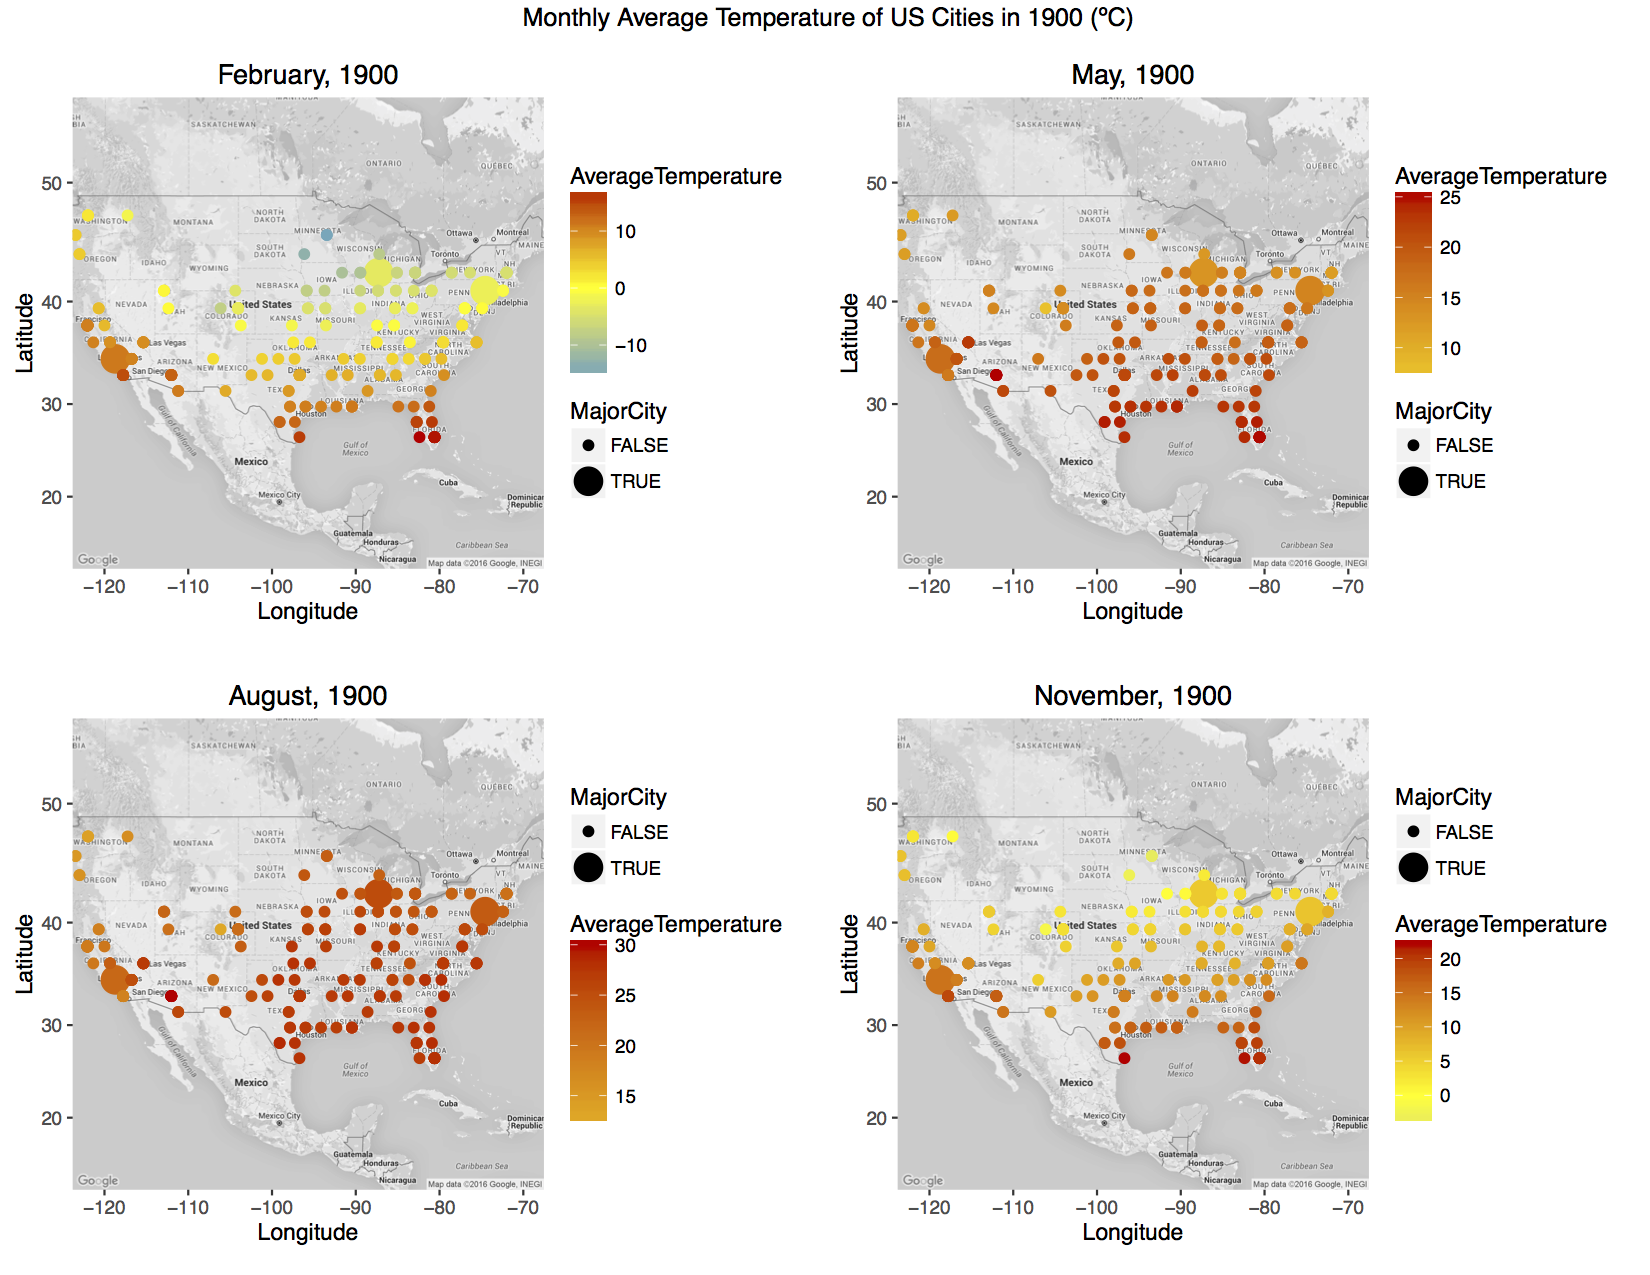
\includegraphics[width=\textwidth]{Figures/1900.png}
    \caption{US City Mid-season Temperatures (year 1900)}
    \label{fig:1900}
\end{figure}

\section{Data}
\subsection{Data Description}
The dataset of global temperatures was collected over 263 years (1750--2012) and downloaded from Berkeley Earth, a non-profit environmental monitoring organization. The dataset contains monthly average temperatures of cities from 243 countries and geographic coordinates of the cities. 

\vspace{0.5cm}
\noindent For the purpose of this study, I subsetted the dataset to include only U.S. city temperatures. As shown in Figure \ref{fig:1900} and Figure \ref{fig:2000}, the mid-season temperatures increased by a noticeable amount between 1900 and 2000. However, this observation alone does not imply the overall rise of U.S. ground-level air temperature nor the presence of a linear trend. Further investigation is needed. 

\begin{figure}[H]
    \centering
    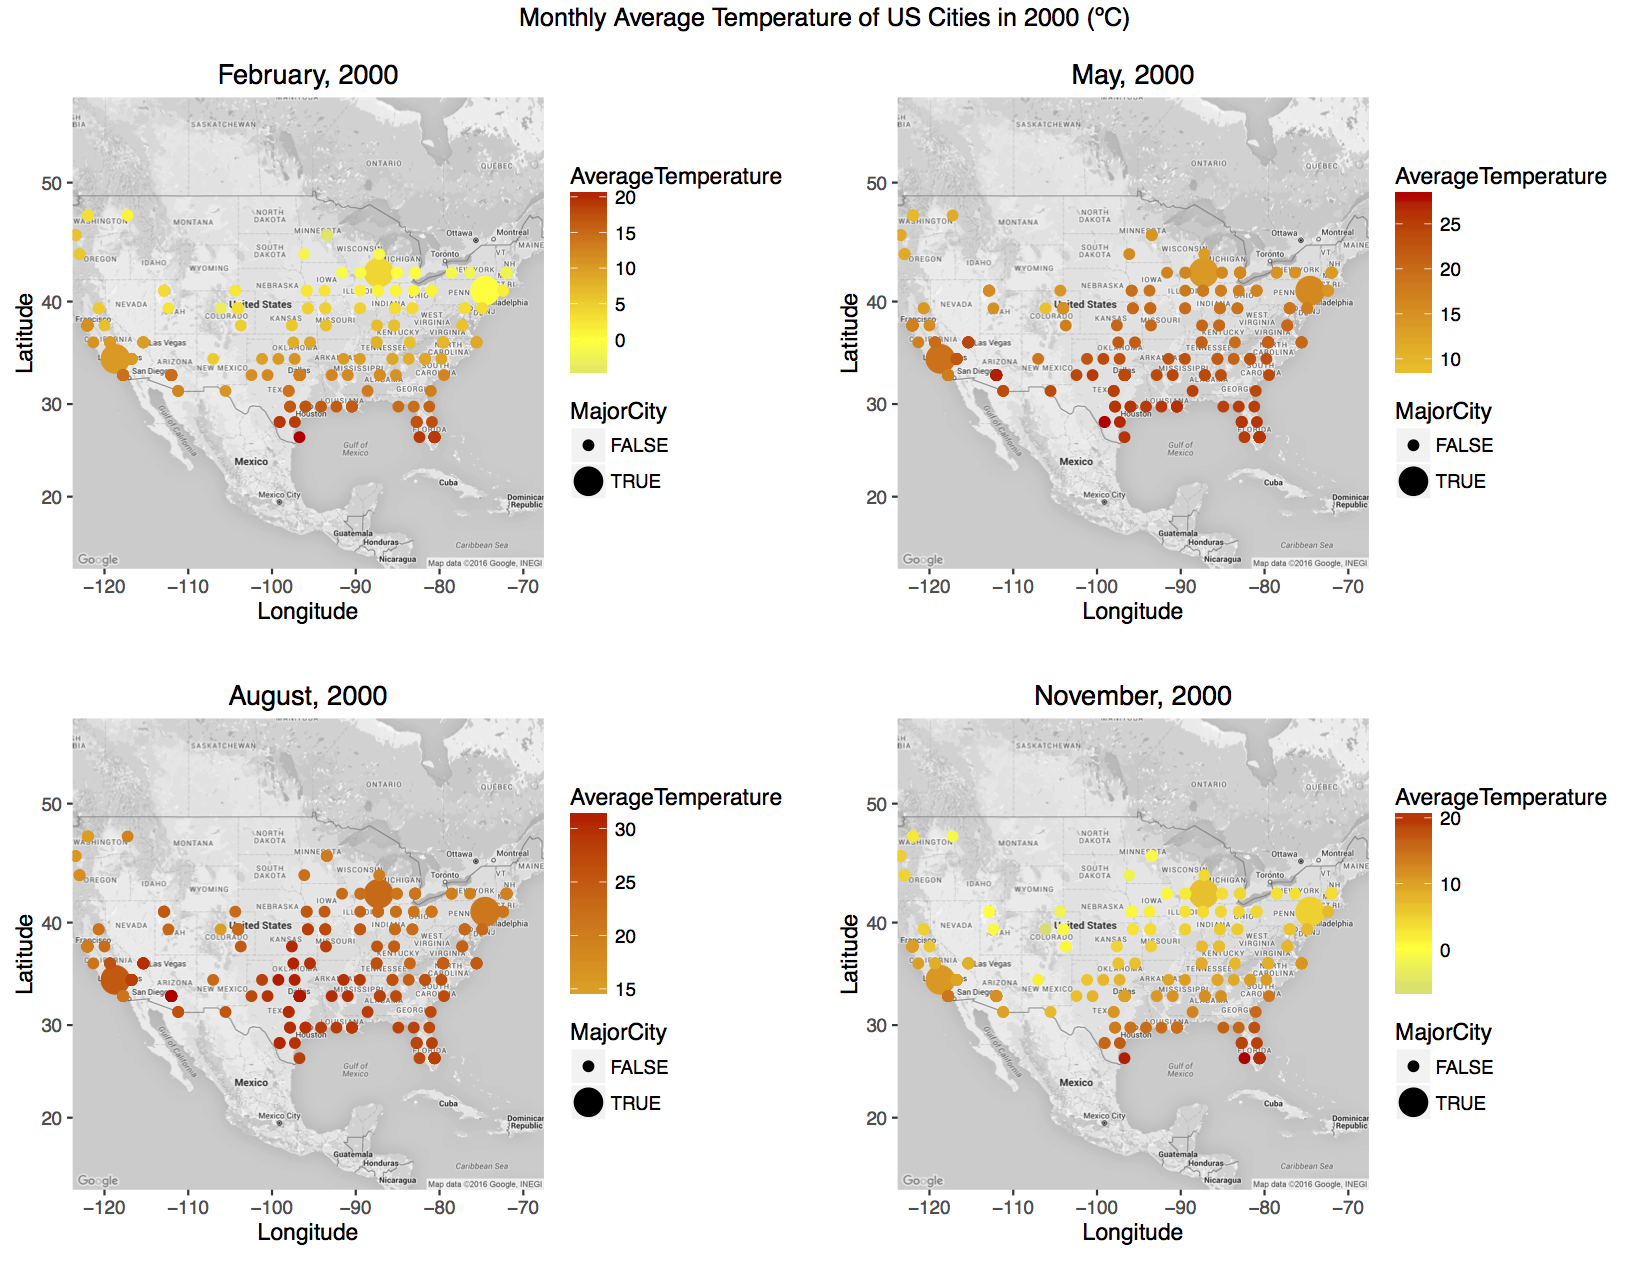
\includegraphics[width=\textwidth]{Figures/2000.png}
    \caption{US City Mid-season Temperatures (year 2000)}
    \label{fig:2000}
\end{figure}


\subsection{Why NYC, LA, and Chicago?}
Due to the high concentration of human activities, global climate change is prominently observed in major cities. Being the three most populated cities in the United States with populations of 8175133, 3792621, and 2695598 respectively \cite{uscb}, New York City, Los Angeles, and Chicago (NYC, LA, and CHI below) might be representative of the other cities in their respective regions in terms of temperature shifts. Furthermore, as shown in Appendix \ref{sec:stateCity}, temperatures of the three cities indeed exhibit the same overall patterns as that of their states. By studying temperature changes in these cities, we might be able to gain certain insights on U.S. regional temperature fluctuations. 




\section{Exploratory Data Analysis}
We start by plotting the raw temperature data of NYC, LA, and CHI (see Appendix \ref{sec:stateCity} and right panel of Figure \ref{fig:citySum}). The line plots reveal that monthly average temperature follows an annual cycle, and the annual cycle oscillates in a not yet clear pattern. Although further testing is required, temperature data for all three cities seems to be stationary (further analysis can be found in the ARIMA section). The histograms in Figure \ref{fig:citySum} resemble the shape of a saddle; notice that the distributions of NYC and CHI temperatures are more spread out while the distribution of LA temperature is more concentrated. Moreover, LA temperature is higher overall, which is to be expected due to its lower latitude. The aforementioned plots indicate the absence of obvious outliers.

\begin{figure}[H]
    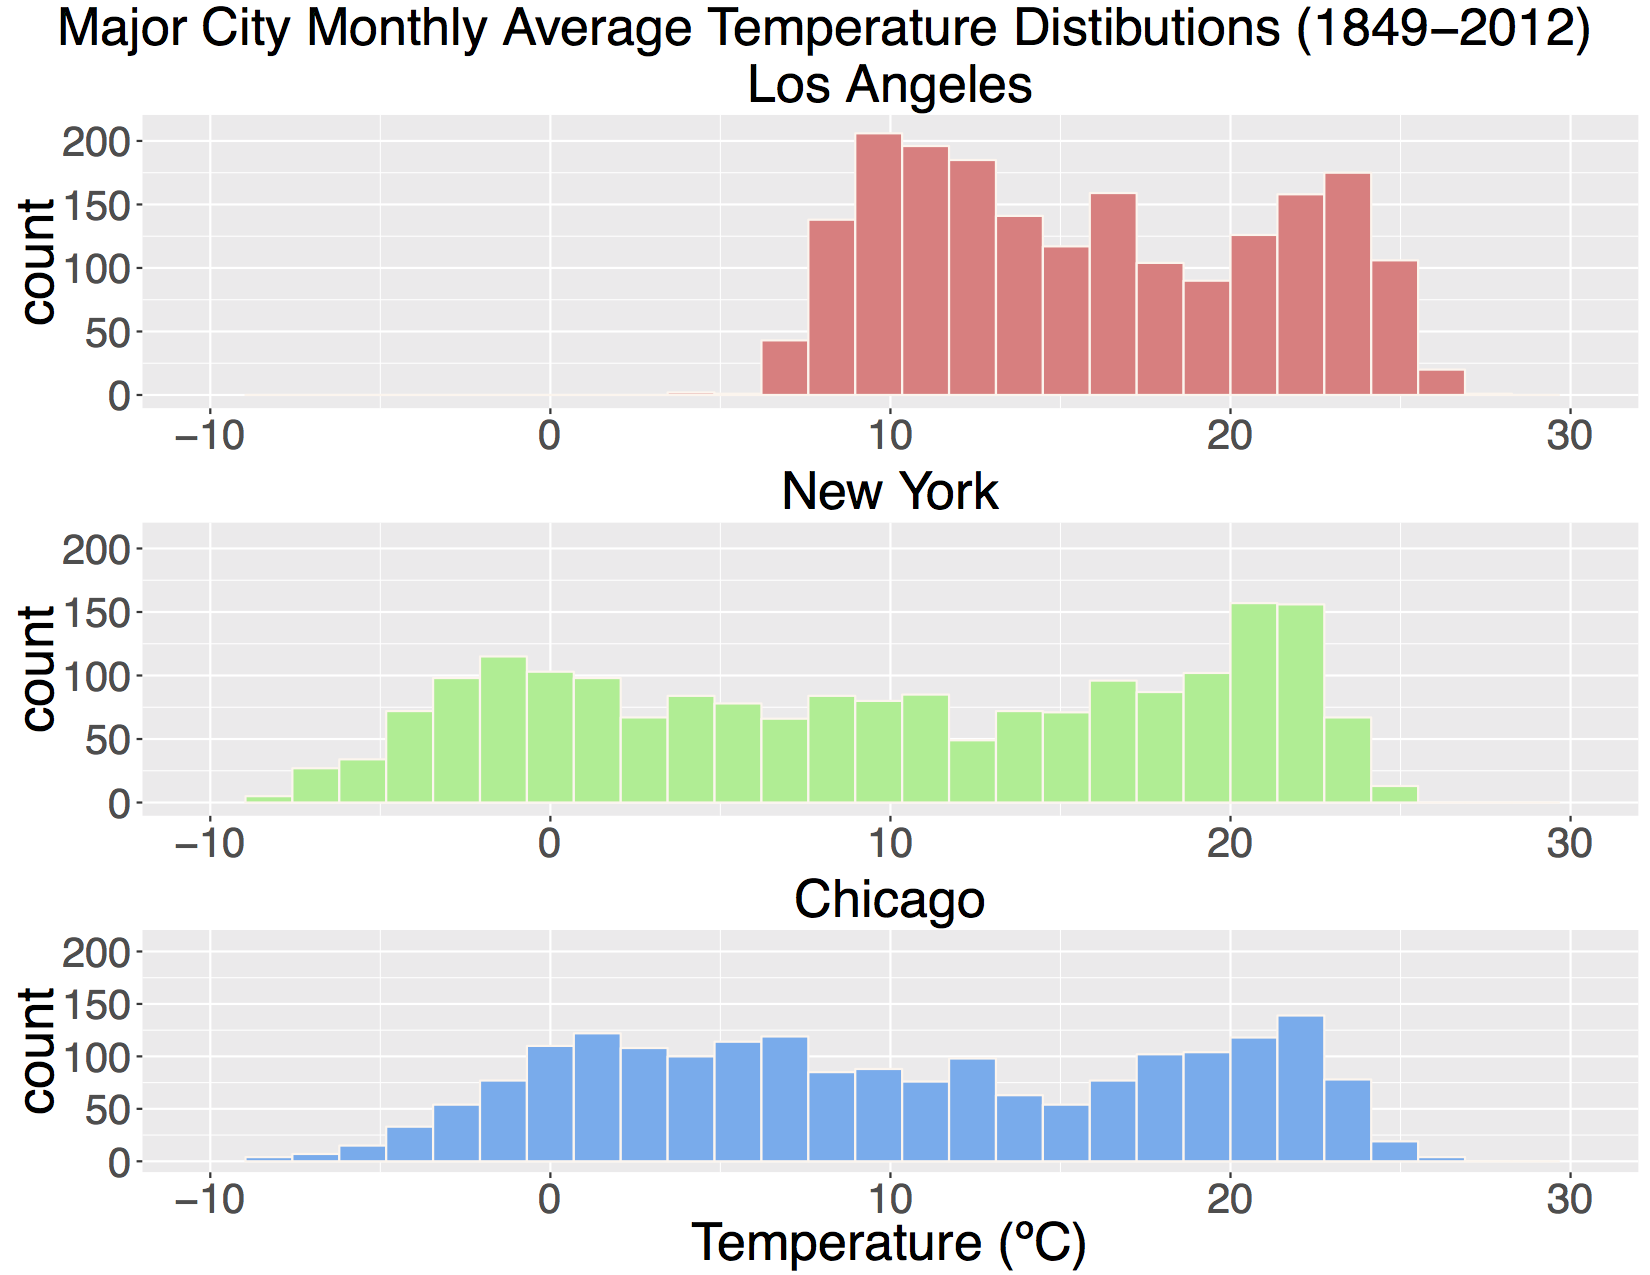
\includegraphics[width=0.5\textwidth]{Figures/cityHist.png}
    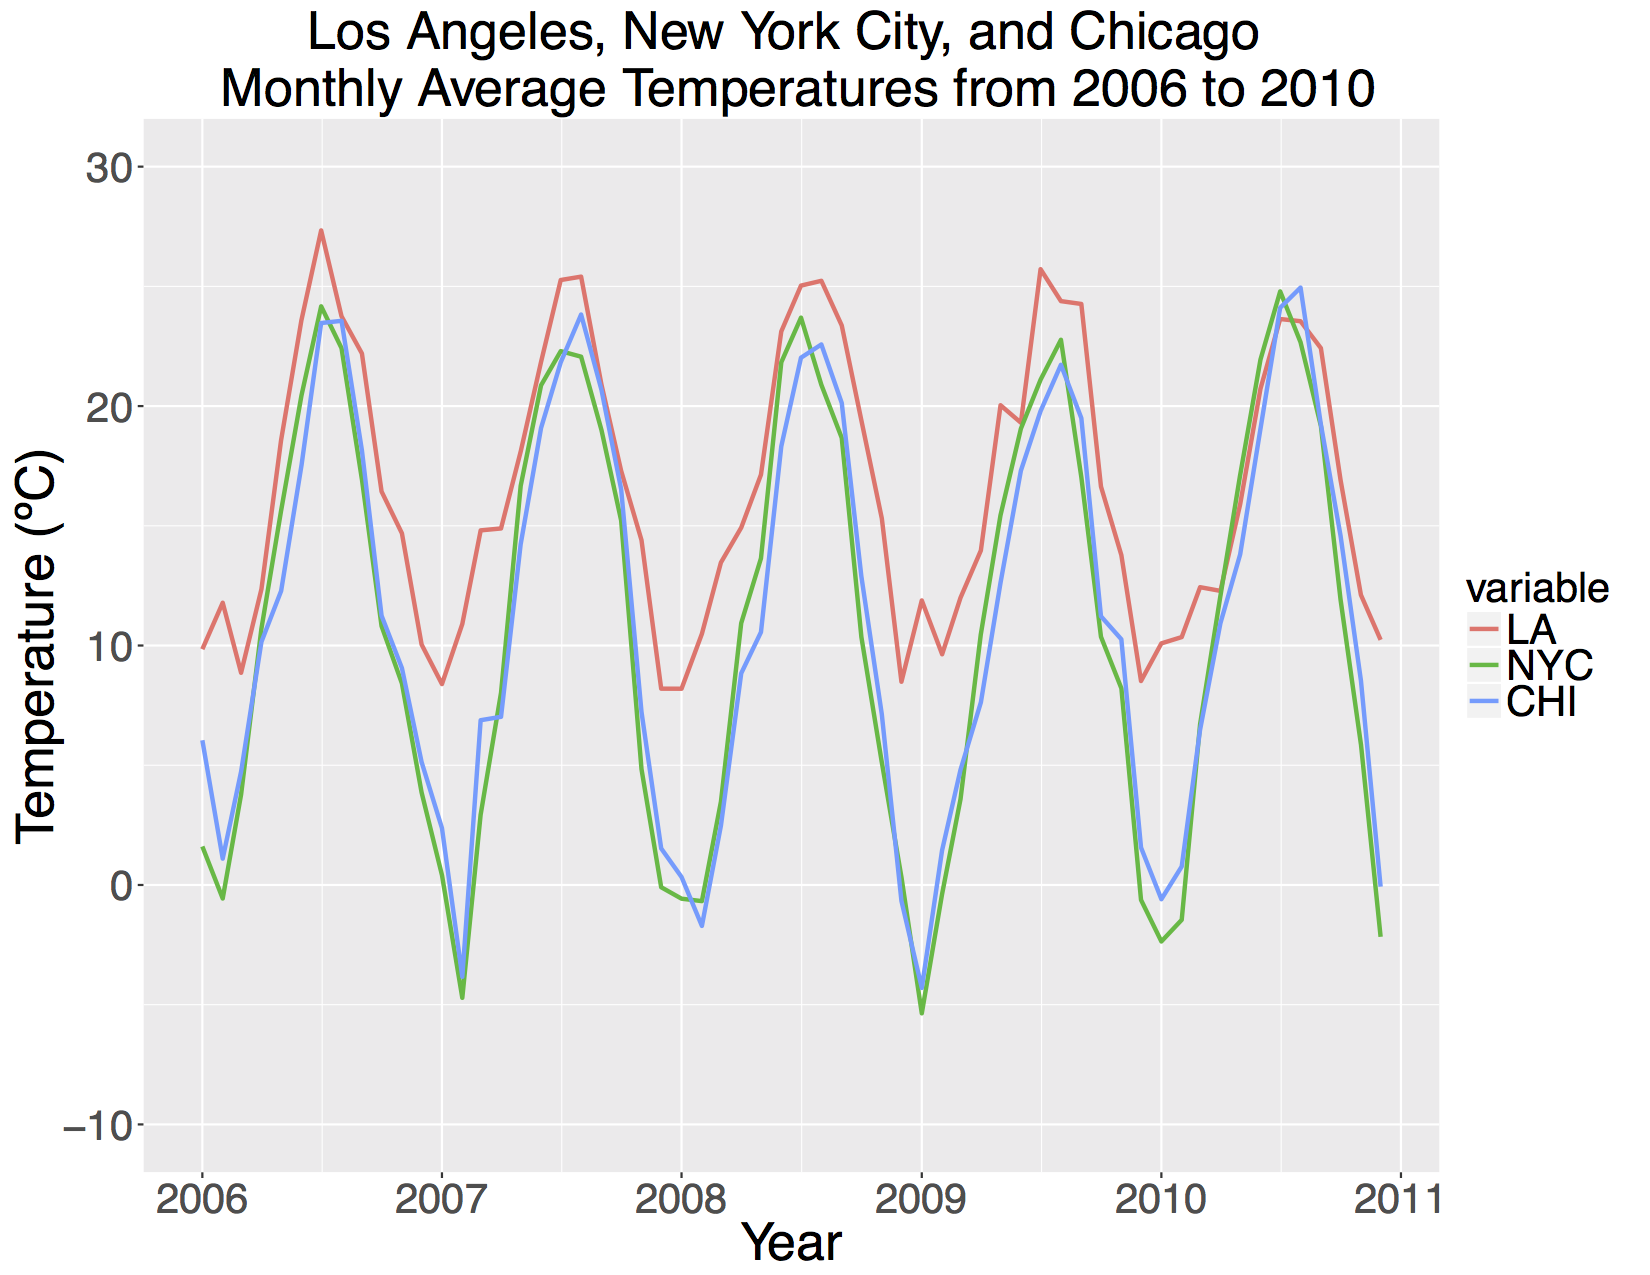
\includegraphics[width=0.5\textwidth]{Figures/cityLine.png}
    \label{fig:citySum}
    \caption{EDA Summary Plots}
\end{figure}


\subsection{Seasonal Decomposition}
To better understand trend and seasonality of the data, we carry out seasonal decomposition on the monthly average temperatures following the model:

\vspace{0.2cm}
\noindent $Y_t = T_t + S_t + R_t$, with $t = 1, 2, ..., (263 yrs * 12 mos)$

\vspace{0.2cm}
\noindent where $T_t$ is the trend component determined using loess regression, $S_t$ is the seasonal component, and $R_t$ is the remainder component. As shown in Figure \ref{fig:laSea}, unsurprisingly, LA temperature data contains a clear annual cycle. The trend component displays a slight upward tendency. Although judging by the sizes of the vertical reference bars on the right side of the plots, the magnitude of the trend was unlikely to be significant. The remainder component resembles white noise which signifies that the majority of the seasonality and trend were successfully captured in the seasonal and trend components. Following the same analysis, similar conclusions were reached for NYC and CHI. Their seasonal decomposition plots can be found in Appendix \ref{sec:sea}.

\begin{figure}[H]
    \centering
    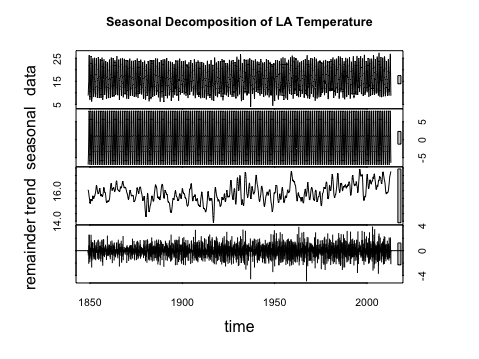
\includegraphics[width=\textwidth, height=9cm]{Figures/laSea.png}
    \caption{LA Temperature Seasonal Decomposition}
    \label{fig:laSea}
\end{figure}




\section{Model Fitting}
\subsection{Linear Regression}
We start by fitting a simple linear regression: 

\vspace{0.2cm}
\noindent $Temp = b_1*Mo_1 + b_2*Mo_2 + b_3*Mo_3 + b_4*Mo_4 + b_5*Mo_5 + b_6*Mo_6 + b_7*Mo_7 + b_8*Mo_8 + b_9*Mo_9 + b_{10}*Mo_{10} + b_{11}*Mo_{11} + b_{12}*Mo_{12} + b_{13}*Yr$, with $t = 1, 2, ..., (263 yrs * 12 mos)$ 

\vspace{0.2cm}
\noindent where $Temp = LA, NYC, CHI$ is the monthly average temperature of the city, $Mo_1, ... , Mo_{12}$ are dummy variables corresponding to the 12 months, and $Yr = 1849, ..., 2012$ is the year. 

\vspace{0.5cm}
\noindent As shown in the table below, p-values of Los Angeles, New York City, and Chicago reveal that regressor $Yr$ is significant at less than the 0.001 level. Since the coefficient of $Yr$ was positive for all three cities, we can deduce a slight upward trend from year to year in average temperature from this model. Upon further inspection, I found that the distribution of the regression residuals is slightly light-tailed (see Appendix \ref{sec:lm} Q-Q plot) but overall close to the normal distribution (see Appendix \ref{sec:lm} histogram). However, the regression residuals displayed a non-random pattern which indicates a poor fit for this linear model (see Appendix \ref{sec:lm} scatter plot).

\begin{center}
    \begin{tabular}{ | c | c | c | c |}
    \hline
    Temp & Coeff. of Yr & p-value of Yr & Adjusted $R^2$ of model\\ \hline
    LA & 0.0047105 & 4.21e-15 & 0.9944  *** \\ \hline
    NYC & 1.047e-02 & $<$ 2e-16 & 0.9848  *** \\ \hline
    CHI & 9.690e-03 & $<$ 2e-16 & 0.9766  *** \\ 
    \hline 
    \end{tabular} \\
    Signif. codes:  0 '***' 0.001 '**' 0.01 '*' 0.05 '.' 0.1 ' ' 1
\end{center}


\subsection{ARIMA}
To improve our linear regression model, we consider adding autoregressive and moving average terms, hence the ARIMA model. 

\vspace{0.5cm}
\noindent To fit an ARIMA model, we first decide whether or not our time series is stationary by inspecting ACF and PACF plots of the series. As shown in Figure \ref{fig:laACF}, LA temperature seems to be stationary. We further test its stationarity by conducting the Augmented Dickey-Fuller test. Since the p-value was less than 0.01, we reject the null hypothesis and conclude that LA temperature data is stationary. Following the same approach, we found that both NYC and CHI temperatures were stationary. Therefore, a differencing term is unnecessary in the ARIMA models (see Appendix \ref{arima} for ACF and PACF plots of NYC and CHI).        

\begin{figure}[H]
    \centering
    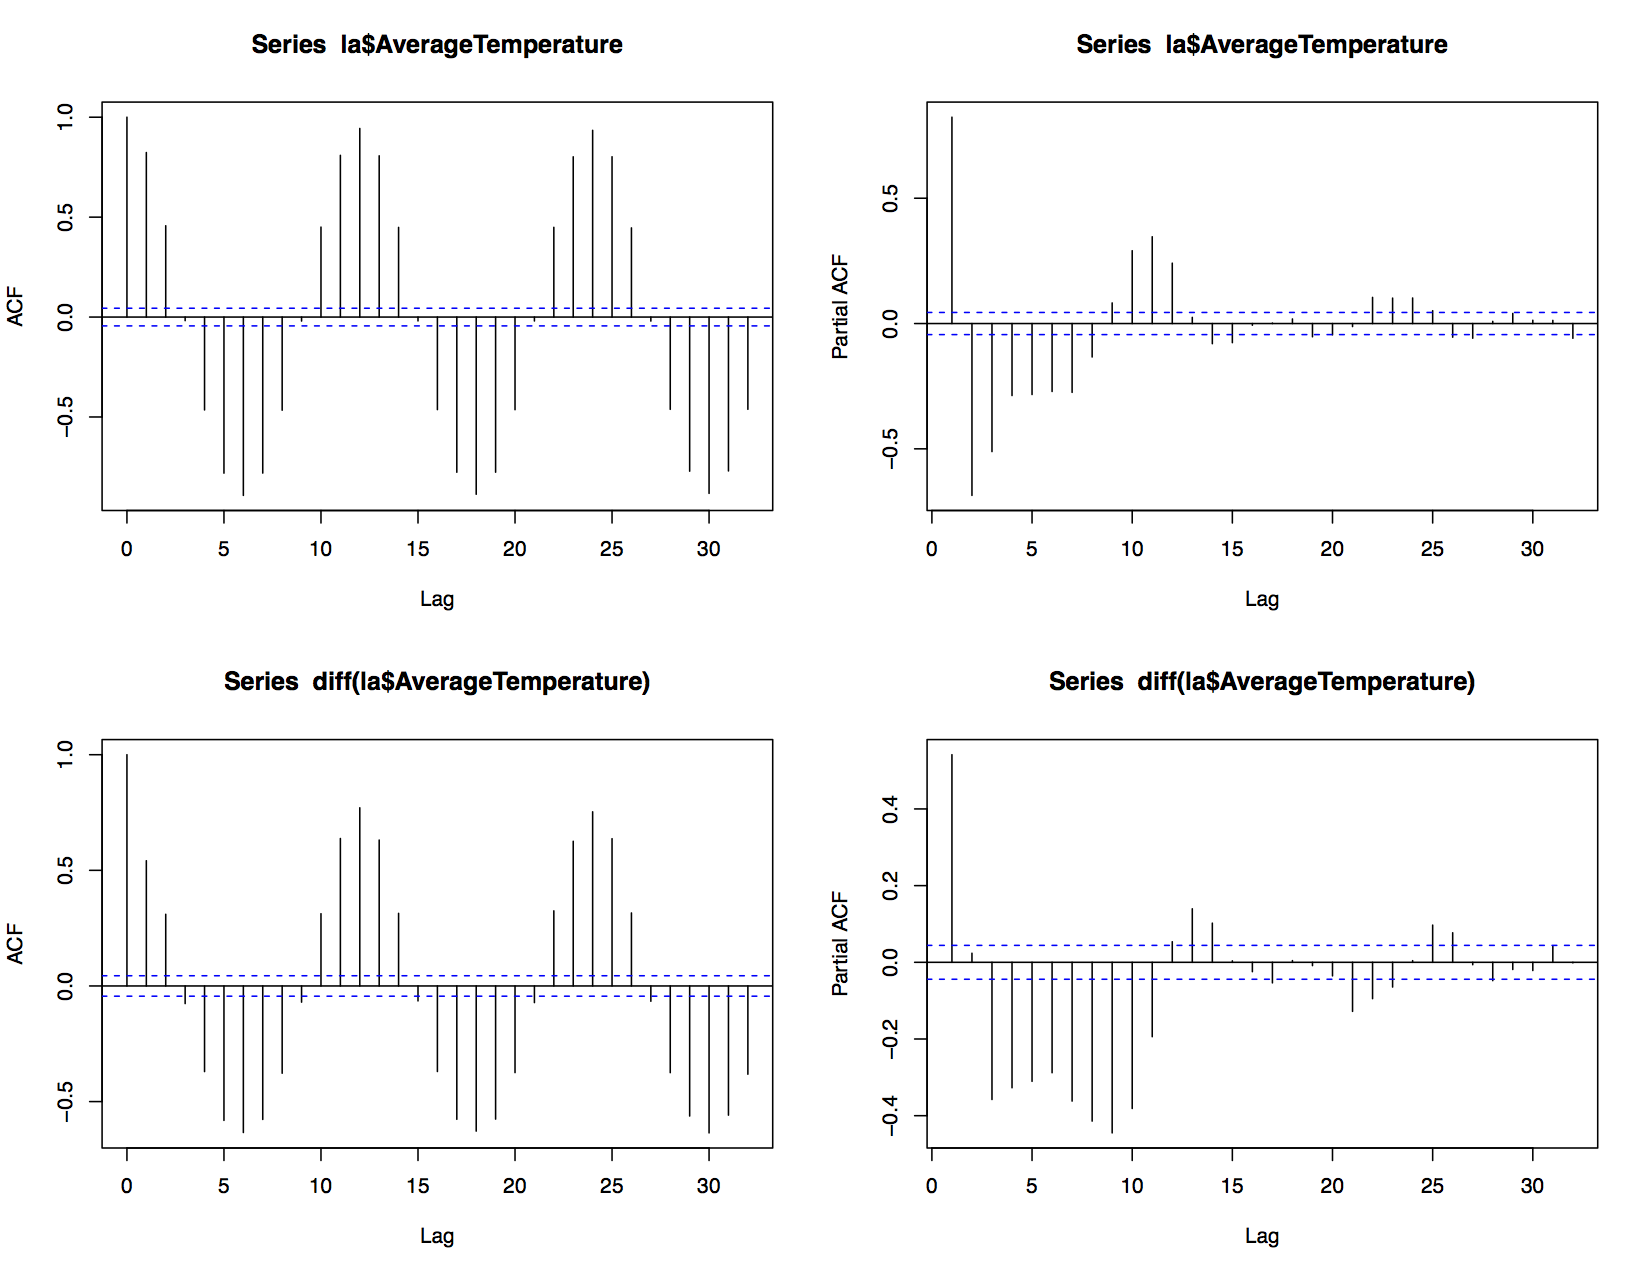
\includegraphics[width=\textwidth]{Figures/laACF.png}
    \caption{ACF and PACF of LA Temperature with and without Differencing}
    \label{fig:laACF}
\end{figure}

\noindent After deciding the order of differencing, we proceed to select the number of AR and MA terms. Since the monthly average temperature data contains a clear annual trend, a seasonal ARIMA model is called upon. Moreover, because the effects of AR and MA terms to some extent cancel each other out, we follow a forward selection process:  after fitting each model, we inspect the ACF and PACF plots of the residuals and decide if additional AR or MA terms are needed. We then take the top 5 possible models and choose the best model based on BIC. Here I used BIC instead of AIC because BIC penalizes overly complex models, which helps prevent overfitting. The selected models for each city along with their BIC's can be found in the table below. To quantify model accuracy, I divided the dataset into a training set (1849-2007) and a test set (2008-2012), using only the training set to fit the model. Next, we analyze the residuals of the selected models by looking at their ACF and PACF plots (see Appendix \ref{arimaRes}) and comparing their distributions to the normal distribution. The Q-Q plot of LA temperature residuals demonstrates that the overall distribution of the residuals is close to the normal distribution though the former is slightly light-tailed. Such a distribution indicates proper selection of the model because the normality assumption was met (see left panel of Figure \ref{fig:laArima}). Q-Q plots of NYC and CHI displayed similar distributions (see Appendix \ref{arimaQQ}). Therefore, the selected models were adequate for our data. 

\begin{figure}[H]
    \centering
    \begin{tabular}{ | c | c | c | c |}
    \hline
    City & Model & BIC & MSE on test set \\ \hline
    
    LA & ARIMA(1,0,1)x(1,0,1) & 6238.159 & 1.568664 \\ \hline
    
    NYC & ARIMA(1,0,1)x(1,0,1) & 7421.719 & 2.963375\\ \hline
    
    CHI & ARIMA(1,0,0)x(1,0,1) & 8191.665 & 4.028274 \\ \hline
    
    \end{tabular}  
    \caption{Selected Models}
    \label{fig:model}
\end{figure}

\noindent Using the selected models, we predict temperature from 2008-2017 and evaluate model performance by calculating the MSEs (see Table \ref{fig:model}). As shown in the right panel of Figure \ref{fig:laArima}, the ARIMA model quite accurately predicted the yearly trend in LA temperature. However, although the MSEs were relatively low, the model did not pick up much of the year-to-year trend.

\begin{figure}[H]
    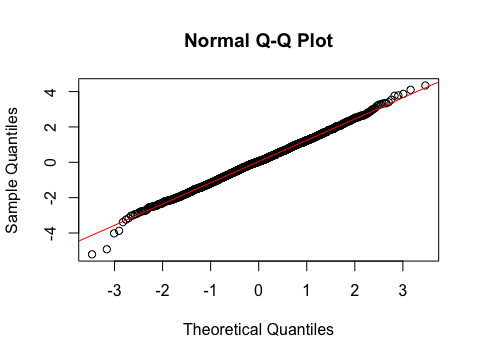
\includegraphics[width=0.5\textwidth]{Figures/laRes.png}
    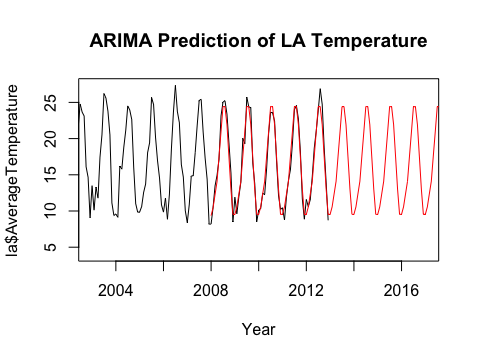
\includegraphics[width=0.5\textwidth]{Figures/laPred.png}
    \caption{Predictions and Residual Q-Q Plot of LA ARIMA(1,0,1)x(1,0,1) (Right panel: black line--real data, red line--prediction)}
    \label{fig:laArima}
\end{figure}


\subsection{Harmonic Regression}
Climate cycles such as $El\ Ni\tilde{n}o$ Southern Oscillation (every 2-7 years) and sunspot cycles (around every 11 years) have been proven to have various levels of influence on global climate \cite{elnino}. To study the effects of the climate cycles, we attempt to perform a harmonic regression which regresses the temperature data on a combination of harmonic (sin and cos) waves. Due to the nature of monthly average temperature data, we should expect the sin and cos waves with one year periods to be important. We also include waves with periods of 1/2-year, 3.5-years, 6-years, and 11-years in order to take into account the effects of $El\ Ni\tilde{n}o$ and sunspot cycles. 

\vspace{0.5cm}
\noindent p-values of the period coefficients indicate that 1/2-year, 1-year, 3.5-year, 6-year, and 11-year periods were significant for NYC and CHI while 1/2 year and 1-year periods were significant for LA (see Appendix \ref{harReg}). Similar to the ARIMA model, we regress on the training set (1849-2007) and predict temperature from 2008-2017. As shown in Figure \ref{fig:laHar}, the harmonic regression produced decent annual predictions of LA temperature, but unfortunately, did not pick up the year-to-year trend. In terms of MSE, harmonic regression performed slightly worse than ARIMA for all three cities. More careful selection of the harmonic waves might help improve the MSEs (see Appendix \ref{harReg}).

\begin{figure}[H]
    \centering
    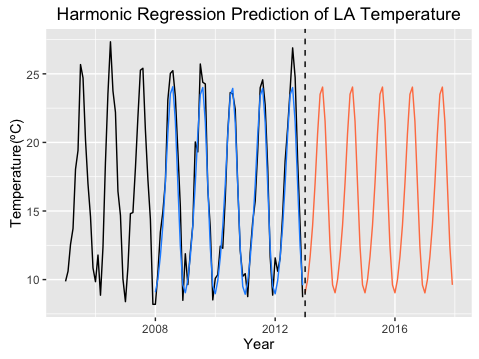
\includegraphics[width=0.5\textwidth, height=6cm]{Figures/laHar.png}
    \caption{Harmonic Regression Prediction of LA Temperature (black line--real data, blue line--prediction on test set, orange line--prediction of the future}
    \label{fig:laHar}
\end{figure}




\section{Spectral Analysis}
To expand on harmonic regression, I conducted spectral analysis on the temperature data by analyzing its periodograms and spectrograms. The theoretical reasoning behind the periodogram is that by fitting N sin waves and N cos waves to data of size N, the regression will perfectly predict the data. Although the regression will be overfitted, it is possible to gain insights on the frequency content of the data by studying which coefficients are significantly different from zero. From the raw log-scaled periodograms, it seems that 1-year, 1/2-year, and 1/3-year periods were significantly different from zero for LA and CHI while only the 1-year period was significant for NYC (see Appendix \ref{sec:period}). However, these raw periodograms are hard to interpret due to high levels of noise. To address this problem, I performed kernel smoothing using Daniell kernels with weighted short moving average ($m=9$). The smoothed periodograms of LA and CHI displayed strong significance for 1-year and 1/2-year periods and mild significance for 1/3-year period while that of NYC displayed strong significance for only 1-year period (see Figure \ref{fig:laSmooth} and Appendix \ref{sec:periodSmooth}); this result is consistent with what the raw periodograms revealed. Additionally, by tapering the smoothed periodograms by 10\% and 30\%, the magnitude of significance for the above periods was made even more prominent (see Appendix \ref{sec:periodTaper}). However, upon inspecting the spectrogram of the continuous Morlet wavelet transform, the majority of LA temperature data only matched the yearly cycle (see Figure \ref{fig:laWave}). Similar results were produced for NY and CHI temperature data. Their spectrograms can be found in Appendix \ref{sec:wave}. 

\begin{figure}[H]
    \centering
    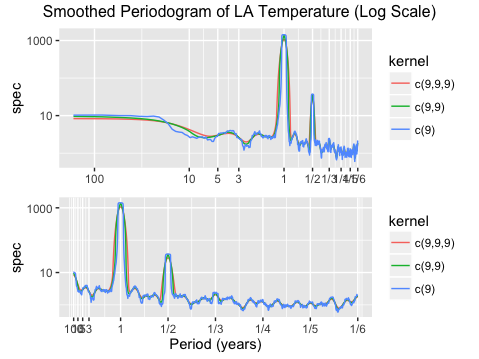
\includegraphics[width=\textwidth, height=9cm]{Figures/laSmooth.png}
    \caption{Smoothed Periodogram of LA}
    \label{fig:laSmooth}
\end{figure}

\begin{figure}
    \centering
    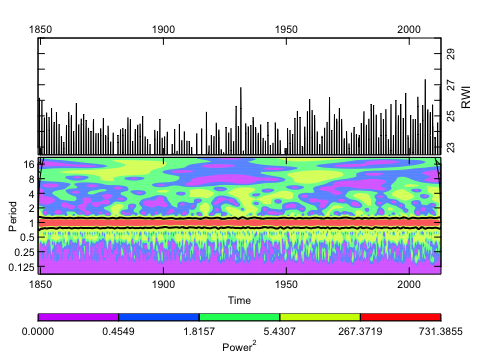
\includegraphics[width=\textwidth, height=9cm]{Figures/laWave.png}
    \caption{Spectral Spectrum of LA}
    \label{fig:laWave}
\end{figure}

\section{Conclusion}
The results from the above analyses demonstrate the predictive ability of time series models---mainly the ARIMA model and the harmonic regression model---on annual ground-level air temperature trends. However, they both failed to capture year-to-year trends, which is more essential for studying global climate change. Results of harmonic regression reinforced the fact that $El\ Ni\tilde{n}o$ and sunspot cycles have significant effects on air temperature over land. Although the linear regression model indicated the increasing trend of temperature from year to year, the results were not conclusive. In future studies, one can improve the harmonic regression model by applying the conclusions from the frequency analysis. In addition, one can examine the relationship between temperature changes and historical events and separate human and nature factors contributing to climate change.




\newpage
\bibliographystyle{plain}
\bibliography{tspaper}
\begin{thebibliography}{9}

\bibitem{suf} 
\textit{Cities and Climate Change}. (2016). Sustainable Urban Futures. Retrieved from \url{http://urban.ias.unu.edu/index.php/cities-and-climate-change}

\bibitem{uscb}
\textit{American FactFinder--Results}. (2014). United States Census Bureau, Population Division. Retrieved from \url{http://factfinder.census.gov/faces/tableservices/jsf/pages/productview.xhtml?src=bkmk}

\bibitem{elnino}
\textit{El Nino, La Nina, and the Southern Oscillation}. (2012). Met Office. Retrieved from \url{http://www.metoffice.gov.uk/research/climate/seasonal-to-decadal/gpc-outlooks/el-nino-la-nina/enso-description}

\bibitem{sats}
\textit{Spectral Analysis of Time Series}. Rstudio Pubs. Retrieved from 

\url{http://rstudio-pubs-static.s3.amazonaws.com/9428_1197bd003ebd43c49b429f22ea4f36e5.html}

\end{thebibliography}




\newpage
\section*{Appendices}
\subsection{State vs Major City Average Temperatures} \label{sec:stateCity}
\begin{figure}[H]
    \centering
    \includegraphics[width=\textwidth]{Figures/stateCity.png}
\end{figure}


\subsection{Seasonal Decomposition}  \label{sec:sea}
\begin{figure}[H]
    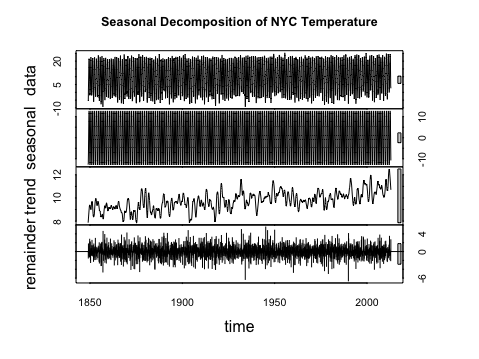
\includegraphics[width=\textwidth, height=9cm]{Figures/nycSea.png}
    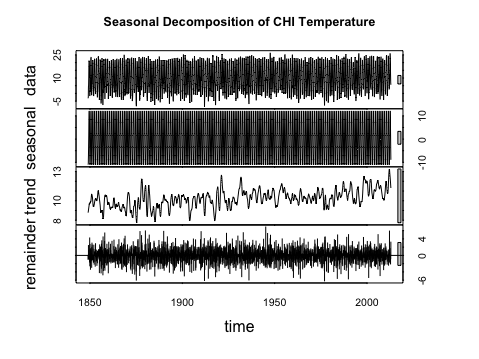
\includegraphics[width=\textwidth, height=9cm]{Figures/chiSea.png}
\end{figure}


\subsection{Linear Regression Residual Analysis} \label{sec:lm}
\begin{figure}[H]
    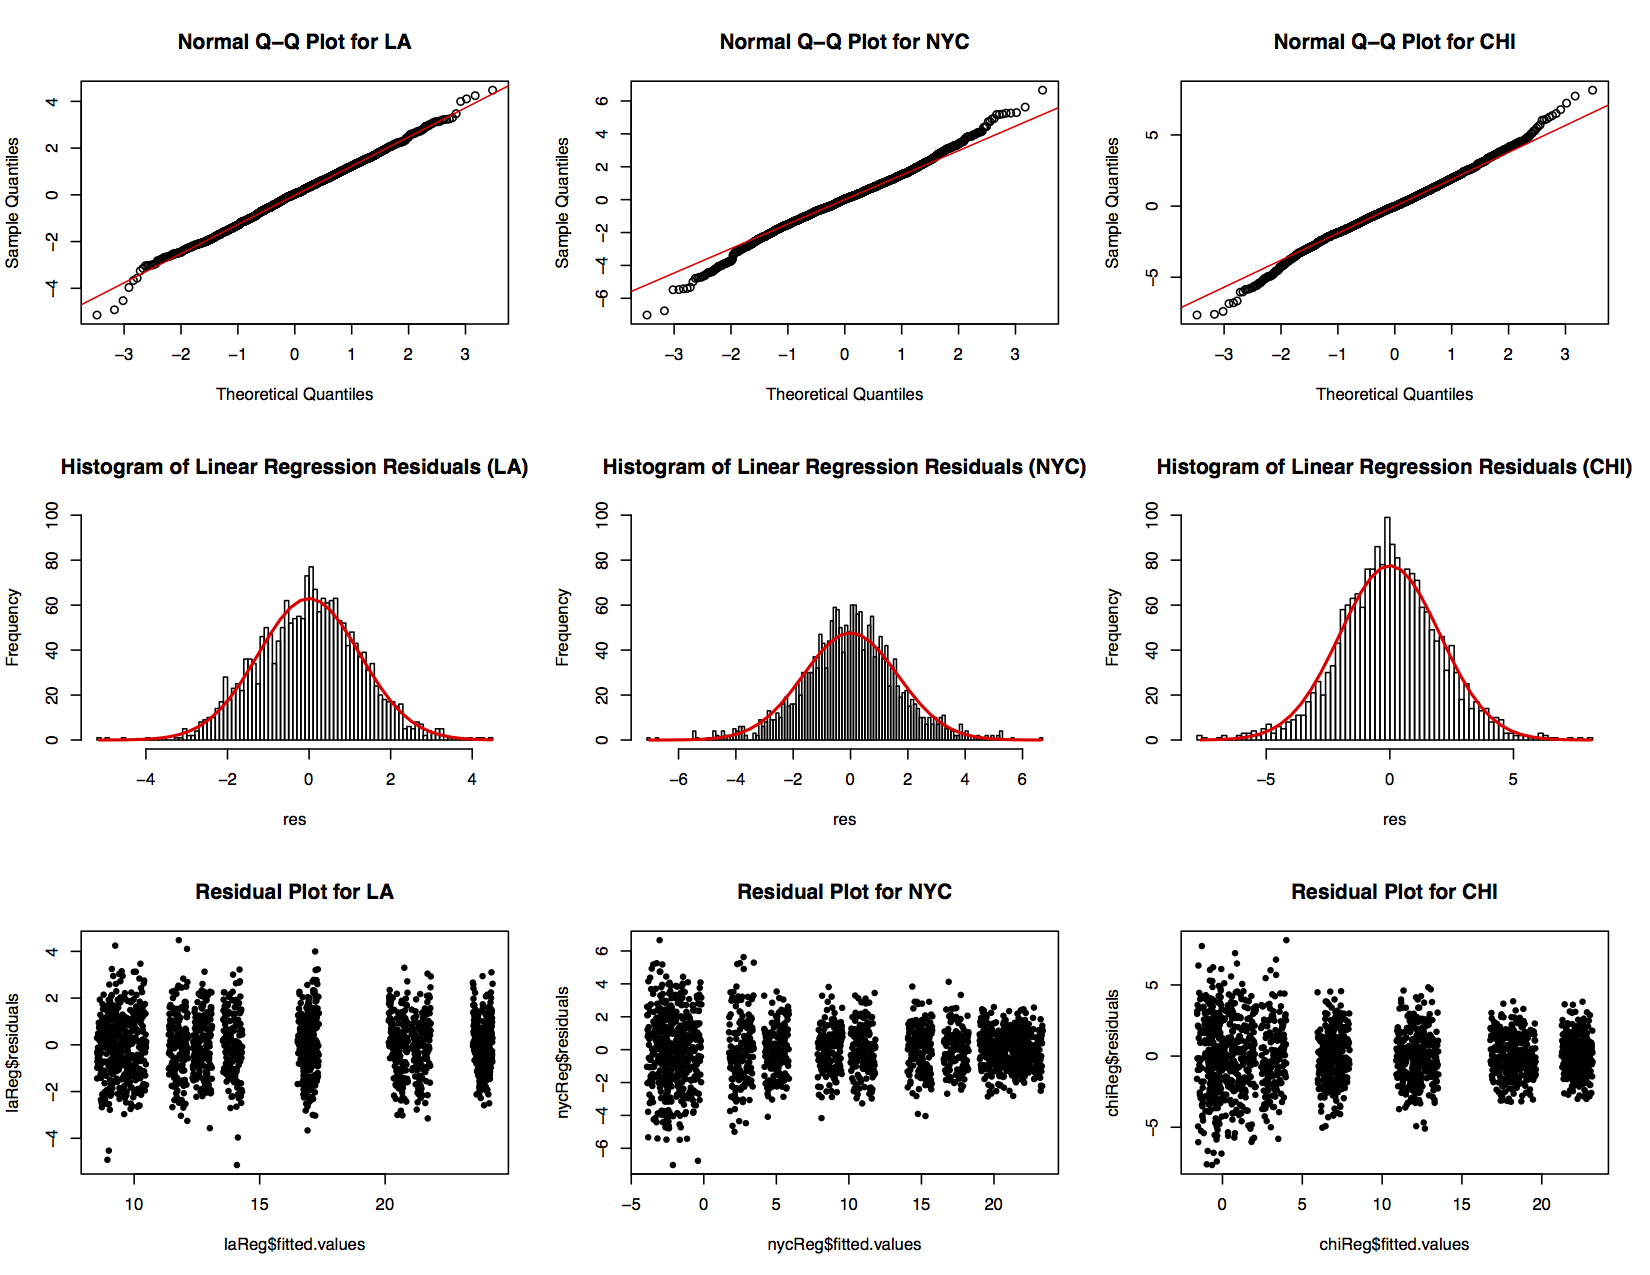
\includegraphics[width=\textwidth]{Figures/reg.png}
\end{figure}


\subsection{ARIMA} 
\subsubsection{ACF/PACF} \label{arima}
\begin{figure}[H]
    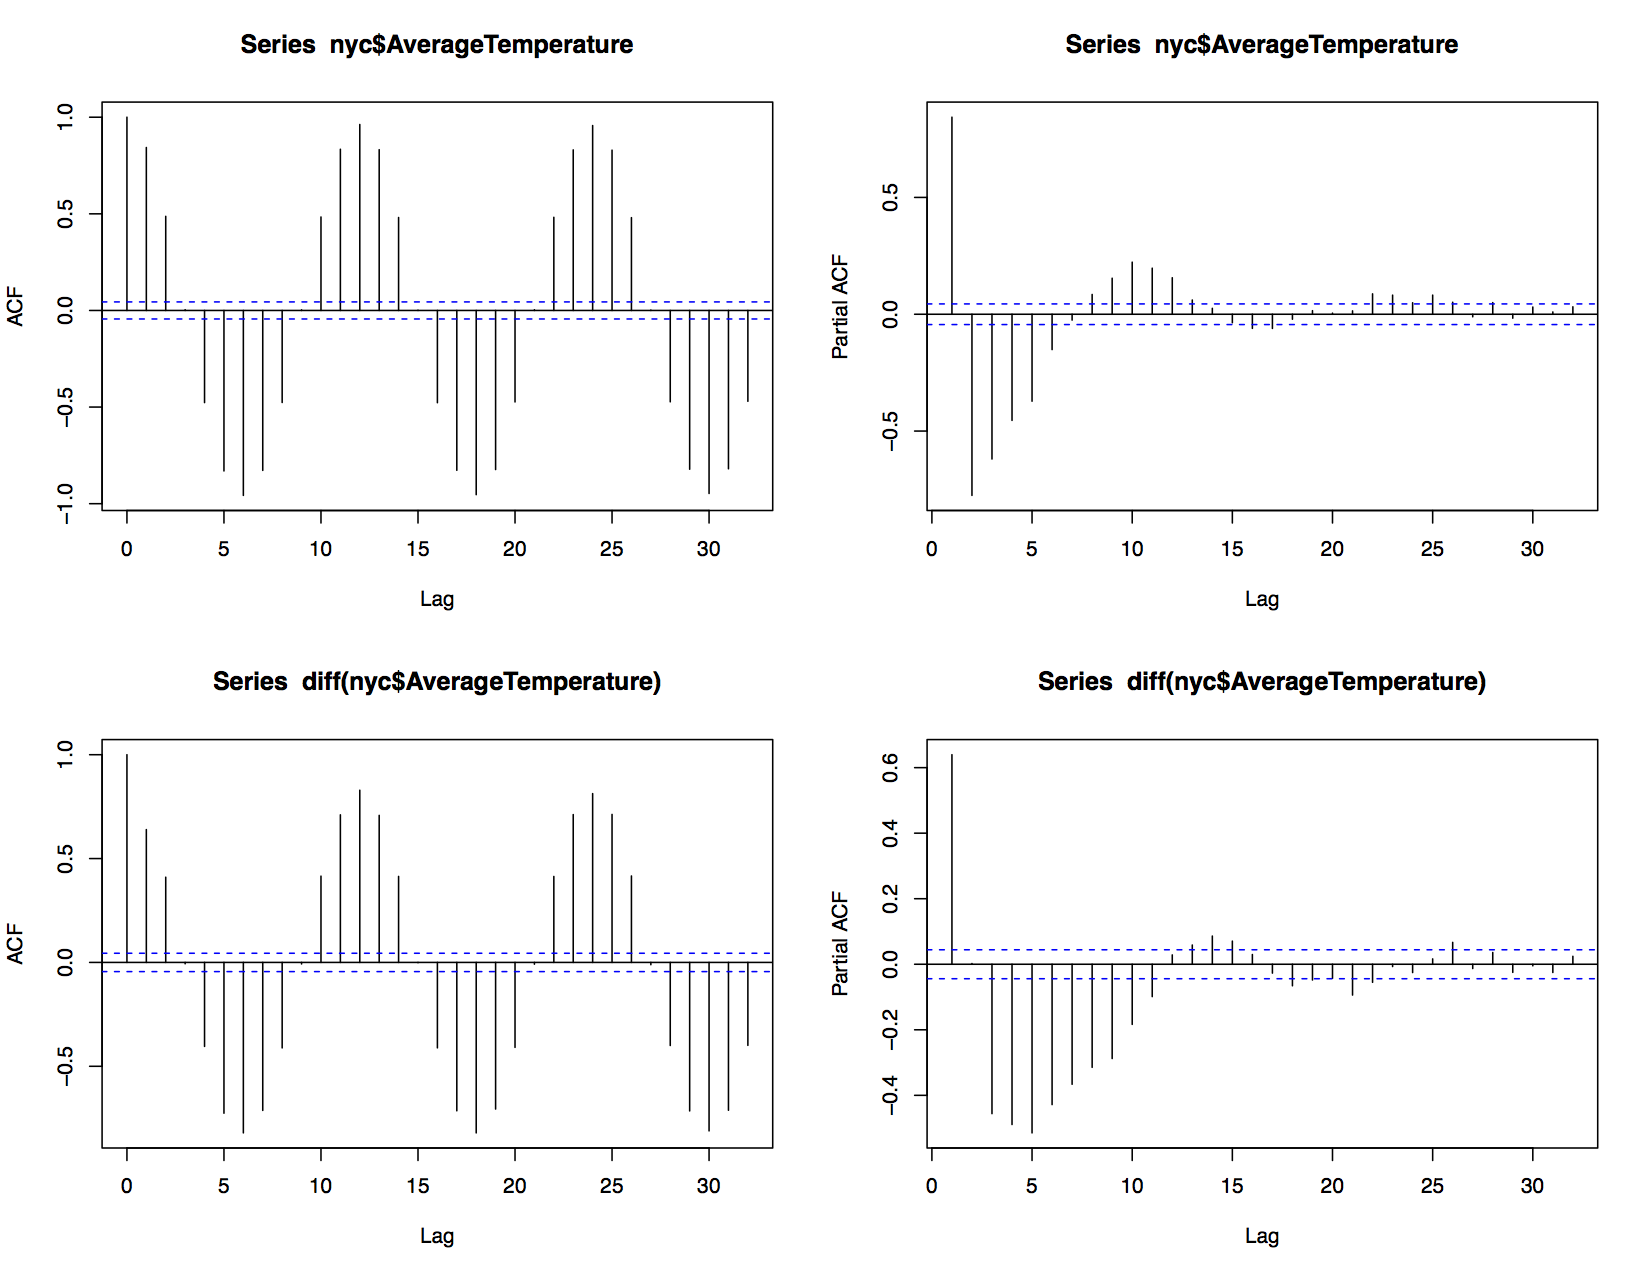
\includegraphics[width=\textwidth, height=8cm]{Figures/nycACF.png}
    \caption{ACF and PACF of NYC Temperature with and without Differencing}
\end{figure}

\begin{figure}[H]
    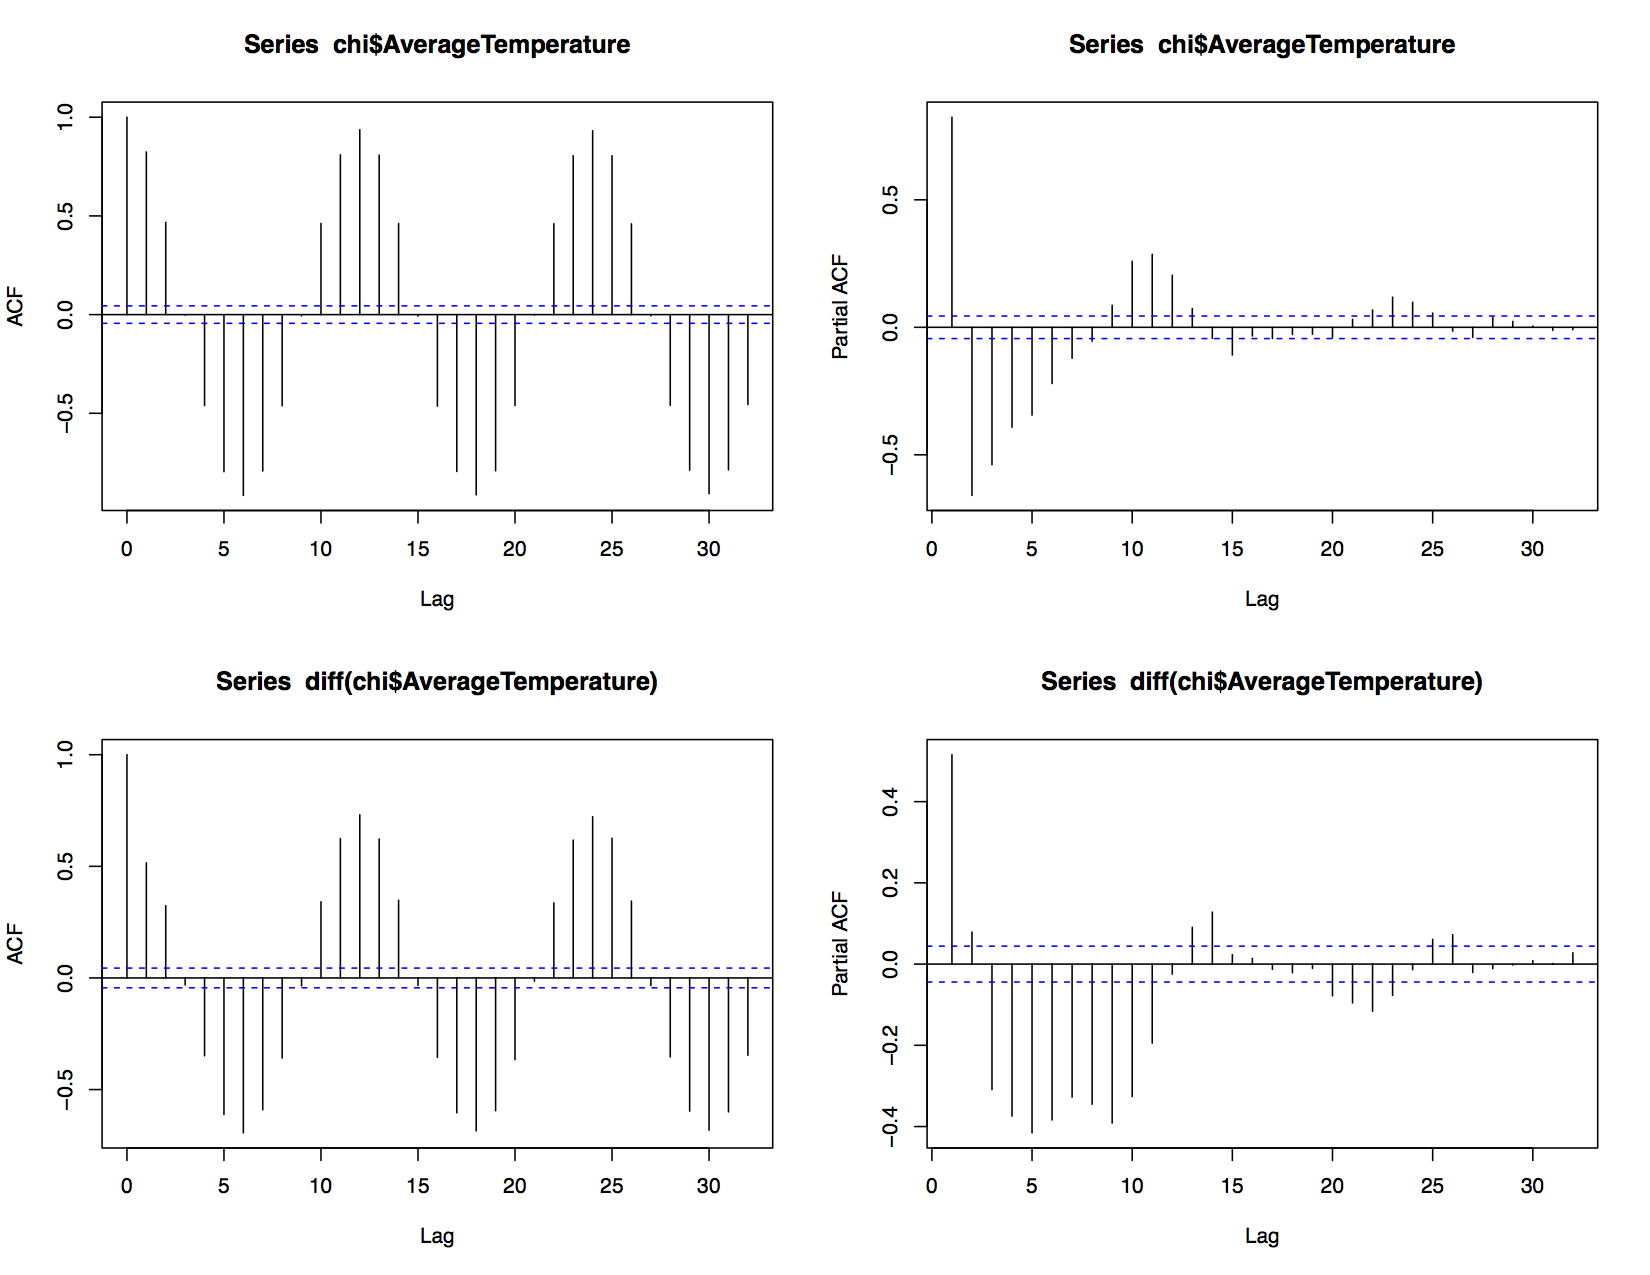
\includegraphics[width=\textwidth, height=8cm]{Figures/chiACF.png}
    \caption{ACF and PACF of CHI Temperature with and without Differencing}
\end{figure}


\subsection{Residual Analysis} \label{arimaRes}
\begin{figure}[H]
    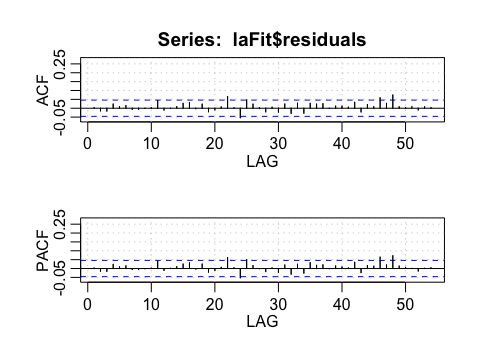
\includegraphics[width=\textwidth, height=8cm]{Figures/laResACF.png}
    \caption{LA ARIMA Residual ACF/PACF}
\end{figure}

\begin{figure}[H]
    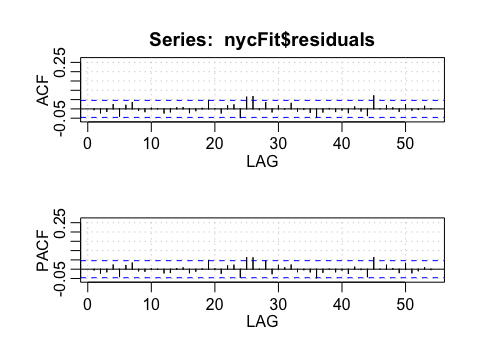
\includegraphics[width=\textwidth, height=8cm]{Figures/nycResACF.png}
    \caption{NYC ARIMA Residual ACF/PACF}
\end{figure}

\begin{figure}[H]
    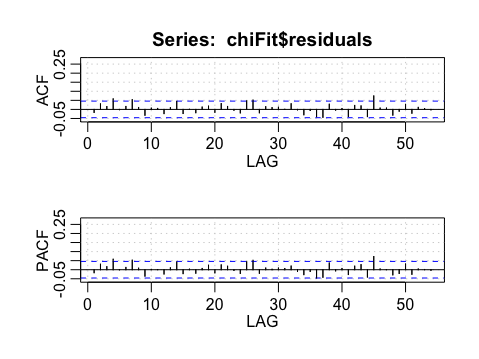
\includegraphics[width=\textwidth, height=8cm]{Figures/chiResACF.png}
    \caption{CHI ARIMA Residual ACF/PACF}
\end{figure}


\subsection{Residual Q-Q Plots} \label{arimaQQ}
\begin{figure}[H]
    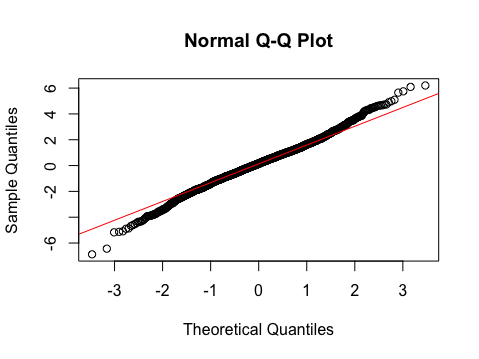
\includegraphics[width=\textwidth, height=8cm]{Figures/nycRes.png}
    \caption{NYC ARIMA Residual Q-Q Plot}
\end{figure}

\begin{figure}[H]
    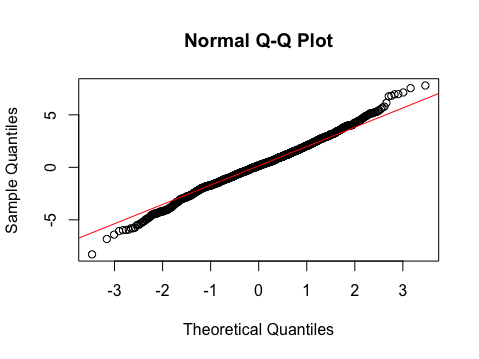
\includegraphics[width=\textwidth, height=8cm]{Figures/chiRes.png}
    \caption{CHI ARIMA Residual Q-Q Plot}
\end{figure}


\subsection{Harmonic Regression} \label{harReg}
\begin{figure}[H]
    \centering
    
    \begin{tabular}{ | c | c | c | c | c | c | c |}
    \hline
    City & 1/2 year & 1 year & 3.5 year & 6 year & 11 year & MSE on test set \\ \hline
    
    LA & \begin{tabular}{@{}c@{}}sin:  $<$2e-16 *** \\ cos: $<$2e-16 *** \end{tabular} & \begin{tabular}{@{}c@{}} $<$2e-16 ***   \\ \ $<$2e-16 ***   \end{tabular} & \begin{tabular}{@{}c@{}}  0.910  \\   0.844  \end{tabular} & \begin{tabular}{@{}c@{}}  0.481  \\   0.508  \end{tabular} & \begin{tabular}{@{}c@{}}  0.467  \\   0.374  \end{tabular} & 2.07559 \\ \hline
    
    NYC & \begin{tabular}{@{}c@{}}sin: 0.320264  \\ cos: 0.000711 ***  \end{tabular} & \begin{tabular}{@{}c@{}}   $<$2e-16 ***   \\    $<$2e-16 ***   \end{tabular} & \begin{tabular}{@{}c@{}}  0.538281  \\   0.066742 .  \end{tabular} & \begin{tabular}{@{}c@{}}  0.157414  \\   0.005573 **  \end{tabular} & \begin{tabular}{@{}c@{}}  0.024862 *  \\   0.280236  \end{tabular} & 4.29451 \\ \hline
    
    CHI & \begin{tabular}{@{}c@{}}sin:  $<$2e-16 ***   \\ cos: 2.13e-05 ***  \end{tabular} & \begin{tabular}{@{}c@{}}  $<$2e-16 ***   \\    $<$2e-16 ***   \end{tabular} & \begin{tabular}{@{}c@{}}   0.130227 \\  0.020551 *  \end{tabular} & \begin{tabular}{@{}c@{}}  0.798048 \\   0.030661 * \end{tabular} & \begin{tabular}{@{}c@{}}  0.000785 *** \\  0.199943  \end{tabular} & 5.162126 \\ \hline
    
    \end{tabular}  \\
    Signif. codes:  0 '***' 0.001 '**' 0.01 '*' 0.05 '.' 0.1 ' ' 1
    \caption{Harmonic Regression p-values and MSEs}
    \label{fig:model}
\end{figure}


\subsection{Spectral Analysis}
\subsubsection{Periodograms} 
\begin{figure}[H]
    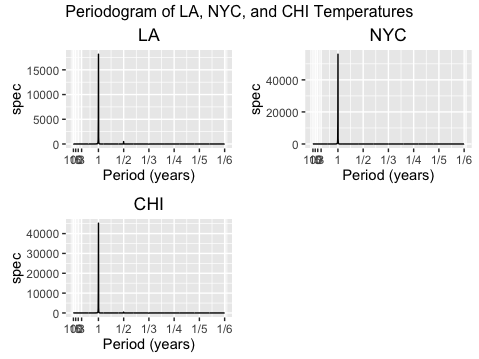
\includegraphics[width=\textwidth]{Figures/cityPeriod.png}
\end{figure}


\subsubsection{Periodograms (Log)} \label{sec:period}
\begin{figure}[H]
    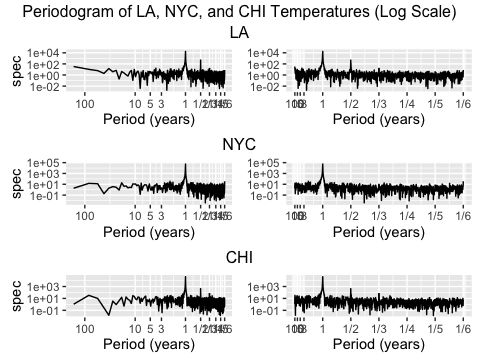
\includegraphics[width=\textwidth]{Figures/cityPeriodLog.png}
\end{figure}


\subsubsection{Smoothed Periodograms} \label{sec:periodSmooth}
\begin{figure}[H]
    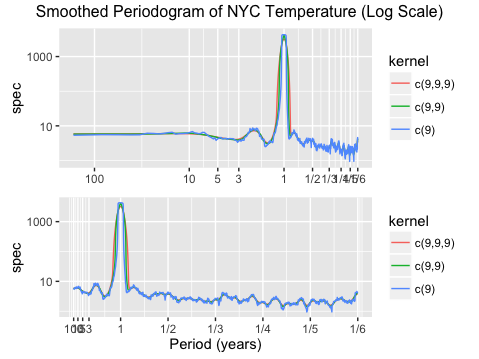
\includegraphics[width=\textwidth, height=9cm]{Figures/nycSmooth.png}
\end{figure}

\begin{figure}[H]
    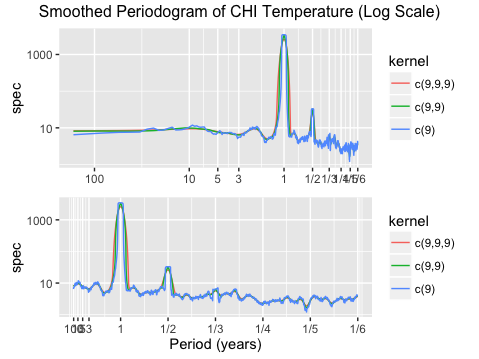
\includegraphics[width=\textwidth, height=9cm]{Figures/chiSmooth.png}
\end{figure}


\subsubsection{Smoothed and Tapered Periodograms} \label{sec:periodTaper}
\begin{figure}[H]
    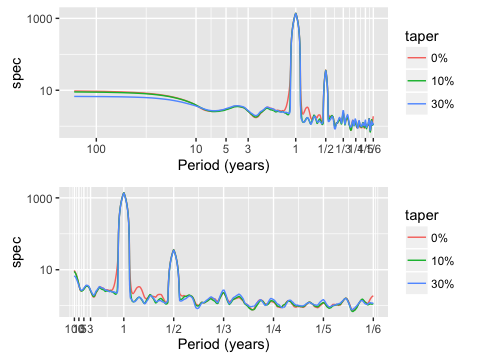
\includegraphics[width=\textwidth, height=9cm]{Figures/laTaper.png}
    \caption{Smoothed and Tapered Periodogram of LA}
\end{figure}

\begin{figure}[H]
    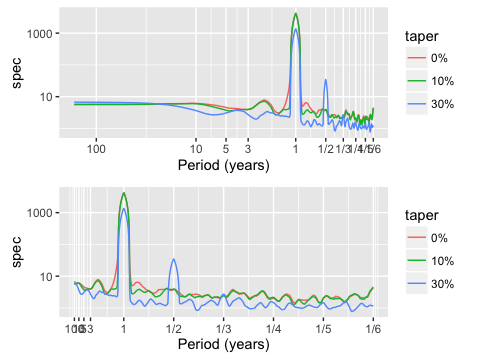
\includegraphics[width=\textwidth, height=9cm]{Figures/nycTaper.png}
    \caption{Smoothed and Tapered Periodogram of NYC}
\end{figure}

\begin{figure}[H]
    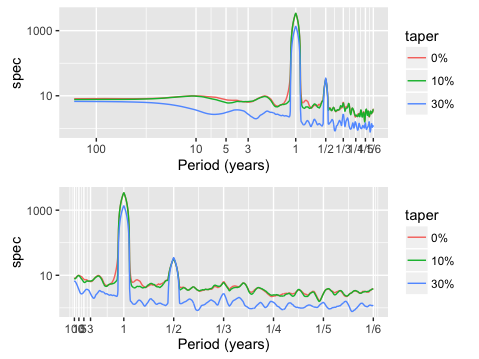
\includegraphics[width=\textwidth, height=9cm]{Figures/chiTaper.png}
    \caption{Smoothed and Tapered Periodogram of CHI}
\end{figure}


\subsubsection{Spectral Spectrums} \label{sec:wave}
\begin{figure}[H]
    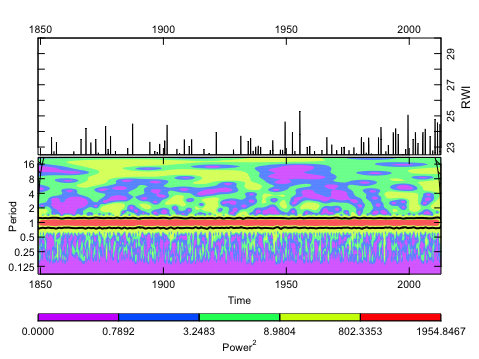
\includegraphics[width=\textwidth, height=9cm]{Figures/nycWave.png}
    \caption{Spectral Spectrum of NYC}
\end{figure}

\begin{figure}[H]
    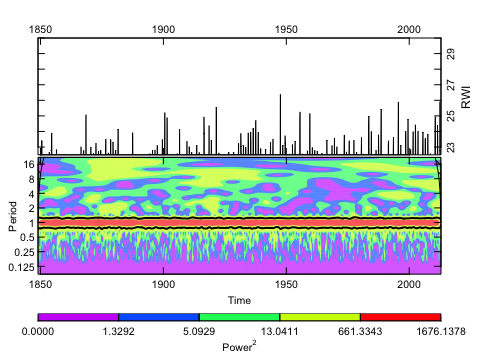
\includegraphics[width=\textwidth, height=9cm]{Figures/chiWave.png}
    \caption{Spectral Spectrum of CHI}
\end{figure}




\end{document}